\chapter{Game Design}

Before we start implementing the game, we should design its individual parts.
An overall design was described in section~\ref{sec:original-vision}.
In this chapter, we will go into more detail and flesh out the design.
We need to decide which mechanics will be in the game and how will the player interact with them.
The game needs to react to the player's actions and communicate the information the player should know.
This all depends on what exactly are we trying to achieve.
Thus, we will start by setting some design goals.

\section{Design goals}

We aim to make the game's mechanics clear, and controls intuitive and responsive.
This is a necessity for every game because without this, the players can't even properly play the game we want them to play.
This is an important goal that will inform many of our decisions throughout the design.

We have analyzed several games of similar genres to our game, that we find enjoyable, and we tried to identify what makes them fun.
We identified five features, which we think make the games very intriguing and replayable, that we think would work for our game too.
Thus, we intend to design the game, so it exhibits these features, making them our game-specific design goals.
We will explain each in a separate subsection, and we will use other games as inspiration for how to reach them.
The goals are:
\begin{enumerate}
    \item \nameref{sec:goal-depth-battle}
    \item \nameref{sec:goal-depth-run}
    \item \nameref{sec:goal-various-builds}
    \item \nameref{sec:goal-force-exploration}
    \item \nameref{sec:goal-challenge}
\end{enumerate}

\subsection{Strategic Depth in Every Battle} \label{sec:goal-depth-battle}

One of the design goals we identified is that the game should let the player make meaningful strategic decisions throughout every battle.
Each battle should be different enough to require the player to adapt to the current situation.
This is where the action will happen, but we want the player to make tactical decisions, not test their reflexes.
With this constraint, battles would be boring if every one played out the same.

In \emph{Plants vs.\ Zombies}, the player wants to plant \emph{Sunflowers} or other \emph{sun}-producing plants.
The more they build their economy, the more plants they can afford in the future.
However, these plants can't kill zombies, so the goal is to spend the bare minimum on defense.
This is a hard problem to solve, since when and where zombies will appear is not completely predictable.
What makes this even more complicated are cheap single-use plants like the \emph{Potato Mine}.
It costs only 25\,\emph{sun} and can kill almost any zombie, where, for example, a \emph{Peashooter} costs 100\,\emph{sun}, but is permanent and able to kill many zombies over the course of a level.
This means the player always has to consider if it's better to place a plant that's the best now or a plant that will be the best in the future.

In \emph{Slay the Spire}, the player has to make a similar decision, but even more often.
Almost every enemy grows stronger over time, or makes the player character weaker as they fight.
This means that the player always has to consider when it's the best to defend and when it's better to attack.
The player can choose to not block some damage now in order to kill the enemy sooner and prevent bigger attacks in the future.
The player also has to plan several turns in advance because many cards have longer lasting effects.
They often have to decide whether it's better to play a card that makes them stronger in future turns, or a card that helps them now.

Every fight is different because every enemy has distinctive behavior.
Some enemies get much more powerful over time, so it is important to kill them quickly.
Others punish the player for attacking them, so the player needs to kill them with precision.
Fights also vary a lot because the player draws their cards in a different order every time.
All this means that the player has something to think about every turn.

Our game will also have economic buildings and instant abilities, so the player has to balance economy and short-term versus long-term defense.
The player will have to survive some number of waves, but they will be able to spend extra materials to mine fuel faster and end the battle sooner.
This is similar to being more offensive in \emph{Slay the Spire}, since the waves of attackers should get stronger at a faster pace than the player's defense.
Each battle will require a different approach, since the waves will be composed of a different set of attackers every time.
We can also vary the nature of a battle by changing up the terrain and making attacker paths different lengths or more numerous.
This might seem like too much, but we want to playtest all these options and possibly cut those, which don't work well.

\subsection{Strategic Depth in Every Run} \label{sec:goal-depth-run}

Another of the design goals is that our game should let the player make meaningful strategic decisions throughout every run and there should be no clear path to victory.
In our game, when the player makes a decision when fighting in a battle, its consequences should be contained mostly within the battle.
This goal refers to the decisions the player will make outside a battle, which affect all future battles.

In \emph{Slay the Spire}, the player needs to improve many aspects of their deck in tandem.
They need to have great defensive cards, cards that can deal with enemies that have a lot of health, cards that can attack multiple enemies at once and more.
The player should also care about the average cost of the cards in their deck.
It is bad when the player wants to both defend and attack on a given turn, but they've drawn only an expensive attack and an expensive defensive card.
It is also suboptimal when the player plays out all the cards they've drawn, but they have leftover energy they didn't spend.
Balancing these aspects of the deck leads to some difficult decisions when picking cards to add.
For example, should the player pick a good defensive card because they are lacking in defense, or should they pick an attack that's just very strong.

We want to balance the battles in a way, which requires the player to have strong blueprints with various qualities.
The players should need good economic buildings, fuel-producing buildings, abilities and towers good at dealing with various kinds of attackers.
They should also have some cheaper towers to build in the first few waves and more expensive towers to build once they produce a lot of material.

In \emph{Slay the Spire}, the player comes across the interesting trade-off between short-term and long-term power even in building their deck.
The player wants cards which will have a great potential to be strong in the future, having great synergy with other cards.
But these cards aren't strong right now and the player needs to survive the next few fights, making them choose cards that are useful immediately, but might not be as powerful later in the run.
As an example we can look at the cards \emph{Iron Wave} and \emph{Double Tap}.

The player starts each run with several copies of cards \emph{Defend} and \emph{Strike} in their deck.
Compared to them, \emph{Iron Wave} is a very cost-efficient card.
As shown in figure \ref{fig:sts-iron-wave-and-double-tap}, it costs 1\,\emph{energy} (displayed in the top right corner of the card), the same as \emph{Defend} or \emph{Strike}.
However, it does almost the same thing as \emph{Defend} \textbf{and} \emph{Strike} combined~--- it deals damage and gives \emph{block} too.
Picking this card can help a lot in the early fights, but it doesn't really grow stronger later in the run.
The card \emph{Double Tap}, on the other hand, is not great at the start.
In essence, it acts like another \emph{Strike} most of the time, and is useful only when the player draws another attack alongside it.
It is however very strong when the deck contains many attacks that cost a lot of energy but deal much more damage.
Then it allows the player to play a powerful attack twice at the cost of only one more energy.

\begin{center}
    \captionsetup{type=figure}
    \begin{minipage}{.25\textwidth}
        \centering
        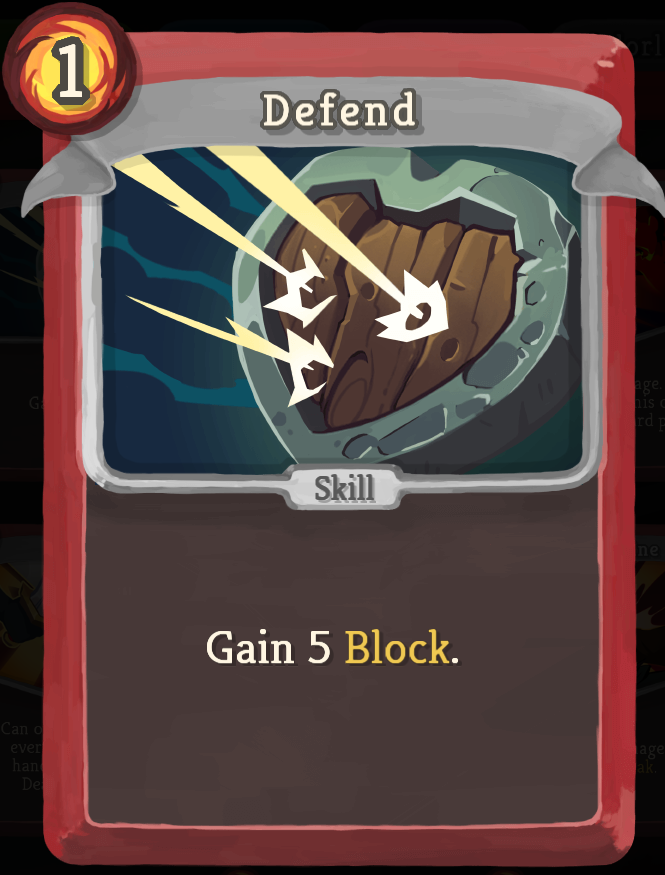
\includegraphics[width=0.95\textwidth]{img/Slay-the-Spire-Defend.png}
    \end{minipage}%
    \begin{minipage}{.25\textwidth}
        \centering
        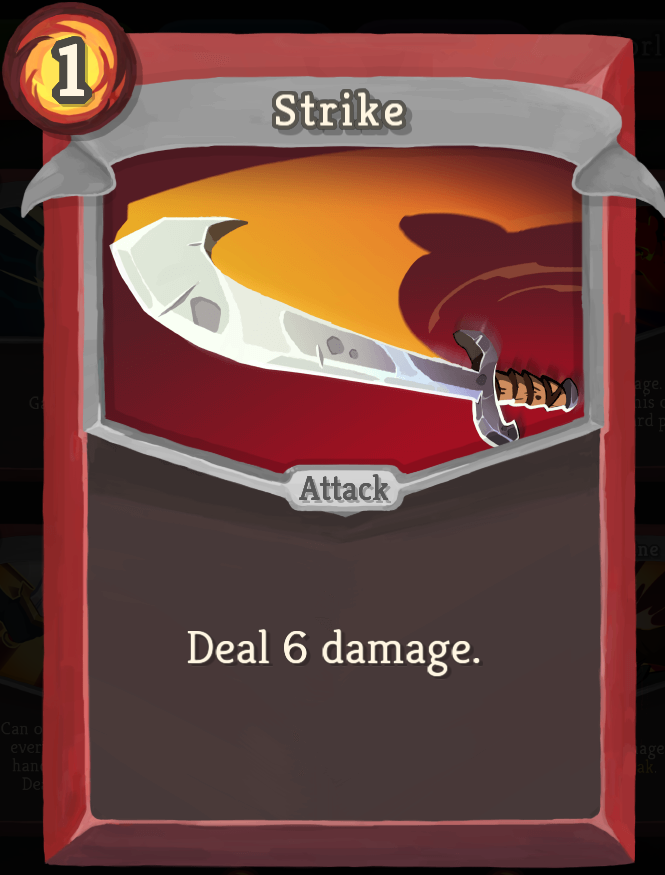
\includegraphics[width=0.95\textwidth]{img/Slay-the-Spire-Strike.png}
    \end{minipage}%
    \begin{minipage}{.25\textwidth}
        \centering
        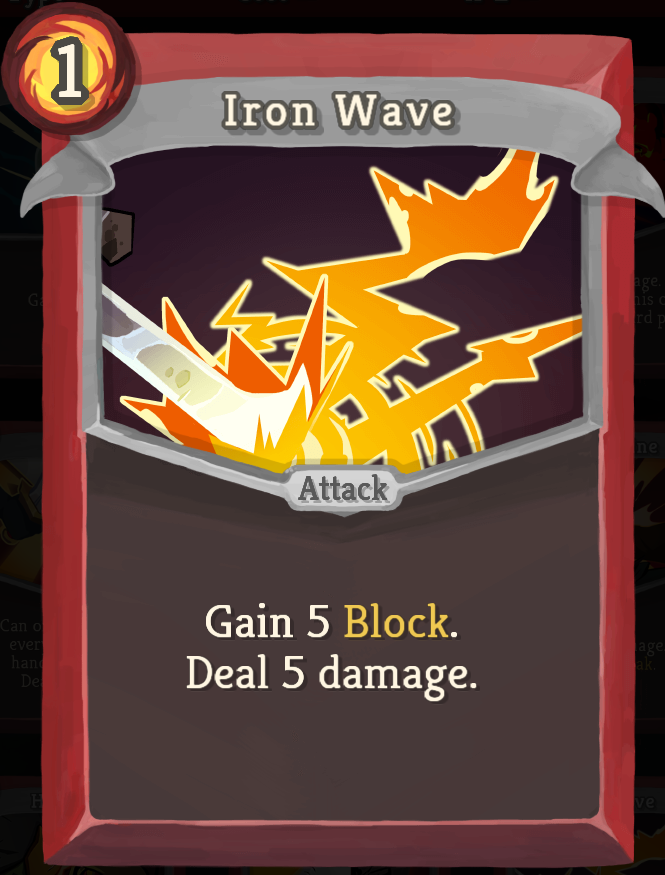
\includegraphics[width=0.95\textwidth]{img/Slay-the-Spire-Iron-Wave.png}
    \end{minipage}%
    \begin{minipage}{.25\textwidth}
        \centering
        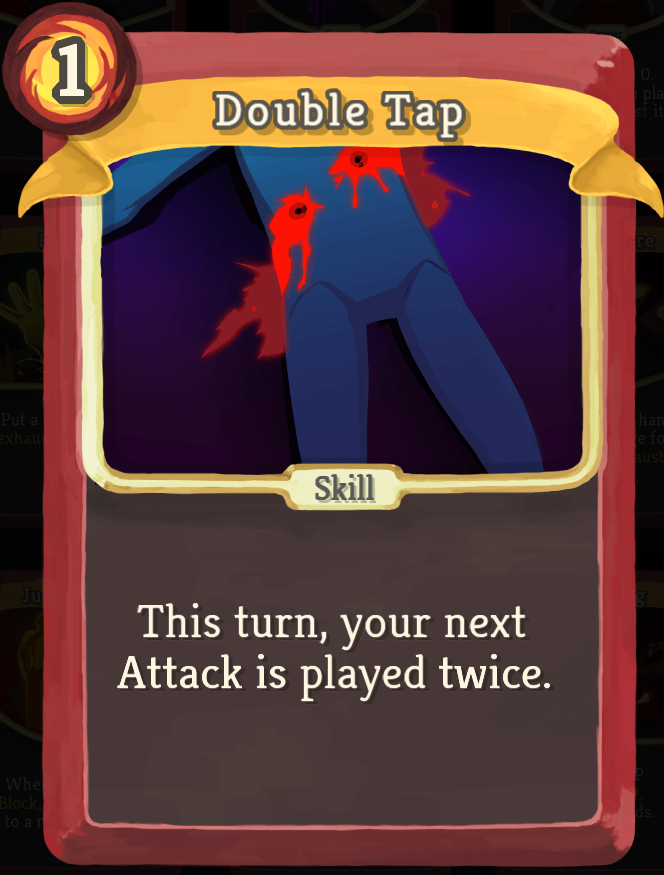
\includegraphics[width=0.95\textwidth]{img/Slay-the-Spire-Double-Tap.png}
    \end{minipage}
    \caption{\emph{Defend}, \emph{Strike}, \emph{Iron Wave} and \emph{Double Tap} cards from \emph{Slay the Spire}.}
    \label{fig:sts-iron-wave-and-double-tap}
\end{center}

We can design the blueprints in our game similarly, making some useful early in the run and some powerful later.
This will let the player decide if they need to take a blueprint that will help them now, or a blueprint that can potentially be strong later.

\subsection{Make Various Builds Viable} \label{sec:goal-various-builds}

One of the goals of our game is that the player should be able to beat the game with a lot of different combinations of blueprints.
We will call these combinations \emph{builds}, as is often done~\cite{buildDict} for unique combinations of skills, attributes and items a player's character can have in a role-playing game.
Builds are distinguished mainly by what they feel like to play with.
If two blueprints are used in the same way, then exchanging one for the other doesn't make a new build.
To allow the player to choose from various builds, there has to be enough blueprints that feel distinct and better yet, they should interact with other blueprints in unique ways.

In figure \ref{fig:pvz-almanac} are shown all the plants from \emph{Plants vs.\ Zombies}.
As we can see, there is a lot of them, and various combinations that work well are possible.
The plants usually don't interact with each other strongly, so the player mostly has to combine the plants such that they have no weak spots.
For example, longer levels require both cheap and expensive defensive plants.
The cheap plants are used at the start of the level, and later they are replaced by the more expensive ones to fit more firepower on the limited lawn.
Some plants can struggle against certain zombie types, so the player also wants to choose plants to cover for all their weaknesses.

\begin{center}
    \captionsetup{type=figure}
    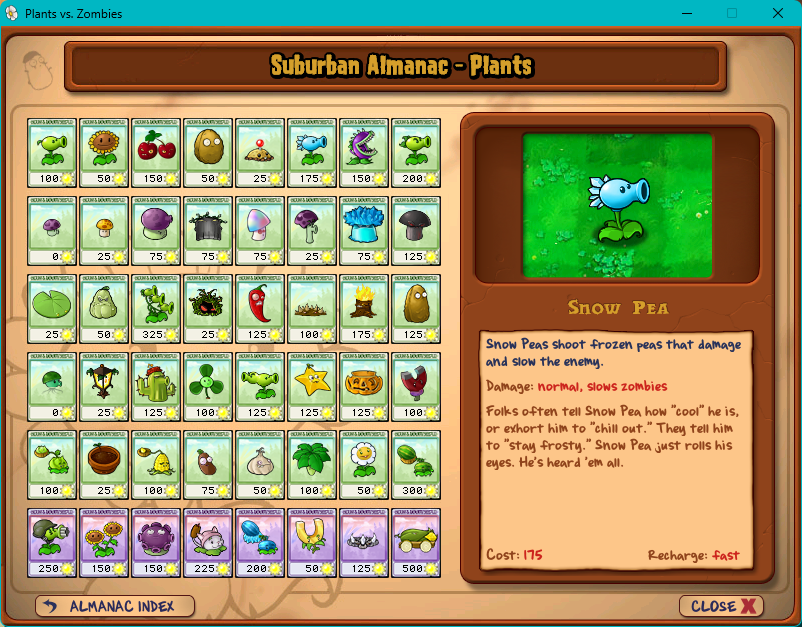
\includegraphics[width=0.8\textwidth]{img/Plants-vs-Zombies-Almanac.png}
    \caption{All the plants of \emph{Plants vs.\ Zombies} in the in-game almanac.}
    \label{fig:pvz-almanac}
\end{center}

We can also look at a few examples from \emph{Slay the Spire}.
Here, builds are often defined by cards that interact in ways that make them stronger.
One of the most blatant examples are cards that apply \emph{poison} to the enemy.
A poisoned enemy takes damage every turn based on the amount of \emph{poison} they have, and the amount decreases by one every turn.
This means an enemy with 2\,\emph{poison} takes $2 + 1 = 3$ damage in total, whereas an enemy with 4\,\emph{poison} takes $4 + 3 + 2 + 1 = 10$ damage in total.
It's easy to see that every card that applies \emph{poison} makes other \emph{poison} cards stronger.

There are also rare cards the player can find, which change how the game works.
For example, defensive cards provide \emph{block} only for one turn because the player character loses all \emph{block} at the start of every turn.
However, once the player plays the card \emph{Barricade}, they don't lose block at the start of their turns for the rest of the fight.
Cards like this can determine the player's strategy for the rest of the game on their own.

We want the players of our game to try lots of different builds and for that, the builds need to be strong enough to beat the game when the player executes them well.
We can tweak the strength of individual blueprints, but we can also design enemies that punish specific builds that would otherwise be too good.
For example, in \emph{Slay the Spire}, many enemies shuffle unplayable cards into the players deck for the duration of the fight.
This punishes decks with fewer cards way more than decks with many cards, keeping small deck builds from being too powerful.

\subsection{Force Exploration} \label{sec:goal-force-exploration}

We don't want the player to just find a single build that works and never explore anything new.
When the player is familiar with a build, it becomes stronger, since they know how to use it effectively.
This discourages them from trying other builds, because they can't use them so well, making them weaker.
Thus, one of our goals is to force the player to explore and make them learn other strategies.

The main way to get cards in \emph{Slay the Spire} are the rewards after every battle, where the player can choose one of three cards to add to their deck, as shown in figure \ref{fig:sts-card-reward}.
All the ways to acquire cards are randomized, so the player can't just hope to always get the card they want.
They have to adapt their build to the cards on offer, so they have to explore different strategies in order to win consistently.
In our game, the player will also pick a blueprint to add to their collection from a randomized offer after each battle.

\begin{center}
    \captionsetup{type=figure}
    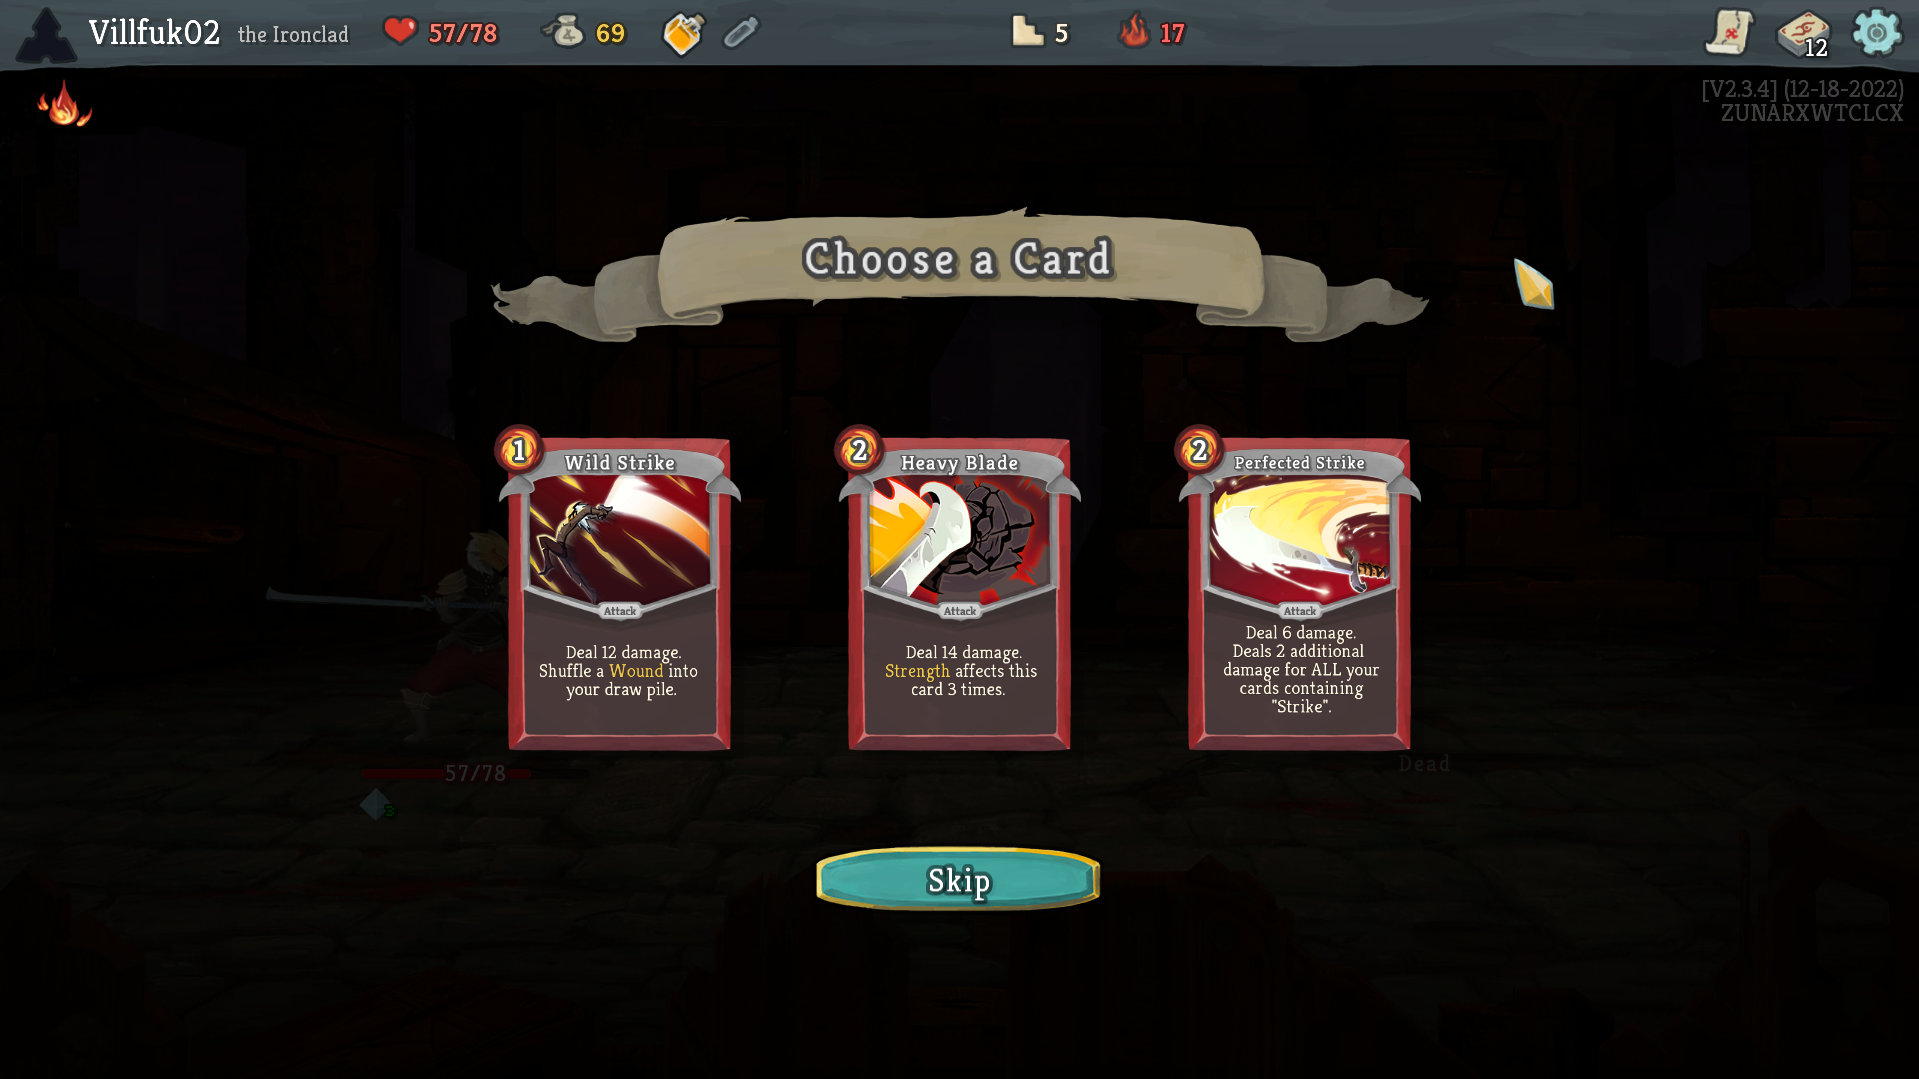
\includegraphics[width=0.8\textwidth]{img/Slay-the-Spire-Reward.png}
    \caption{Card reward screen in \emph{Slay the Spire}.}
    \label{fig:sts-card-reward}
\end{center}

In \emph{Plants vs.\ Zombies}, the player has to adapt to different zombies and level environments.
This can be illustrated with figure \ref{fig:pvz-roof}, which shows a seed select screen.
Here, the player selects which plants they want to use in this level from the selection on the left side.
On the right the player can see that this level takes place on the roof and the zombie types that will appear in this level.
In rooftop levels, the player has to place a \emph{Flower Pot}, which costs 25\,\emph{sun}, on a tile before they can place a plant there.
Furthermore, all plants that shoot in a straight line are of little use here because the roof slopes up, so their projectiles can't travel very far.
An experienced player will also notice that \emph{Bungee Zombies} will appear.
These zombies swing from above to take the player's plants instead of coming from the right.
The player should consider all these factors when choosing the build to play this level with.

\begin{center}
    \captionsetup{type=figure}
    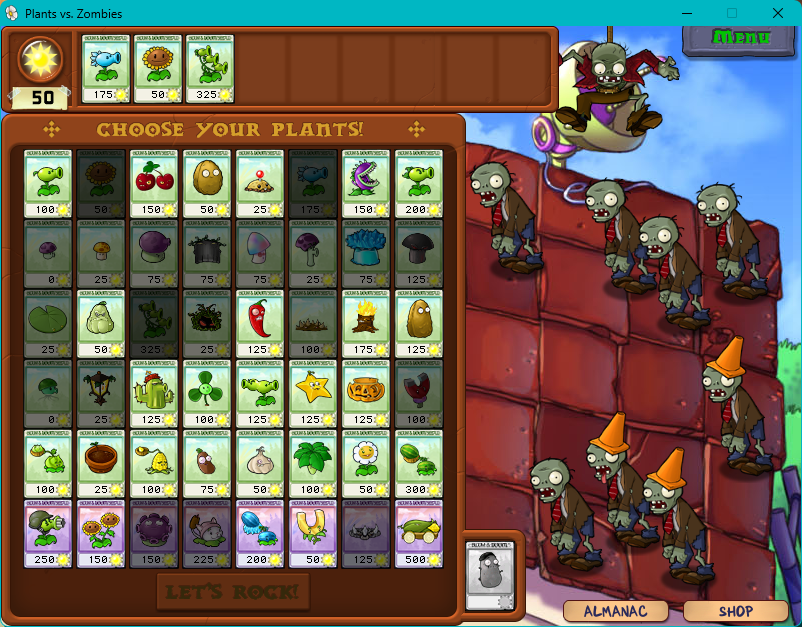
\includegraphics[width=0.8\textwidth]{img/Plants-vs-Zombies-Rooftop.png}
    \caption{Seed select screen in a rooftop level in \emph{Plants vs.\ Zombies}.}
    \label{fig:pvz-roof}
\end{center}

In our game, the player could select which blueprints to play with before every battle based on the level's features and attackers.
Instead, we chose an approach more similar to \emph{Slay the Spire}~--- the player will keep the blueprints they collect for the rest of the run, and they won't know the specifics of a battle before selecting it.
However, they will be allowed to have only a limited amount of blueprints at once, so they still cannot just keep all the blueprints they encounter.

\subsection{Provide a Challenge} \label{sec:goal-challenge}

The player should always have some goal to work towards, just out of their reach.
If the game is too easy, the players will have no reason to think strategically or learn.
Always having a harder challenge to overcome will motivate the player to improve and keep playing.

\emph{Slay the Spire} is not easy to beat, but the player can still improve so much even after beating the game.
After beating the game, the player unlocks so-called \emph{ascension}.
Before embarking on another run, the player can select the \emph{ascension} level they want to play on.
Each level introduces a small change that makes the game slightly more difficult.
Each \emph{ascension} level is unlocked only after the previous level is beaten, and each difficulty increase is small, so it doesn't discourage the player.
These changes are cumulative, so in the end it takes serious effort and luck to beat the game on \emph{ascension} level~20 even for the most skilled players.

This system is simple, yet effective, so we might as well use it too.
We will also want to balance the base game, so that most players that try are able to beat it, but it still takes some effort and several attempts, so the players feel like they've accomplished something.

\section{Procedural Generation}

Randomized procedural generation is of the defining features of the roguelike genre.
We want to use randomized procedural generation to make each run of the game unique.
Since we design the procedural generation algorithms ourselves, we have great control over the results.
However, procedurally generated parts of the game can be really hard to balance.
We need to make sure the randomized parts of the game feel fair to the player.
It doesn't feel good if the player loses the game because they were just unlucky and couldn't have done anything to prevent the loss.
Another issue with randomized procedural generation is that things might start to feel very homogenous.
For example, hand-crafted levels can have features that really stand out.
We need to decide which parts of our game will be procedurally generated and to what degree.

The overall structure of each run will be decided by what we call the \emph{map}.
As stated before, it will be a graph, and the player will go from node to node along the edges.
Each node will be a battle, shop or an event.
We really want each run to be different enough, that the player doesn't develop a single strategy to use in every run.
Since the player will decide where to go, it's not a problem when some paths through the map are more difficult than others.

Every battle will also be randomized to a large degree.
The world a battle takes place on will be procedurally generated, making for a different environment every time.
However, the combination of features that can appear in a given world will be decided by the world's \emph{terrain type}.
There will be several hand-crafted terrain types to randomly select from, some appearing only early in the run and some only later.
This is to create several cohesive styles of the worlds that look and play distinctly from each other.
We feel this is better than if we just let the world generator mix all the features every time, because the results would be more homogenous.
We will go into more detail about the world generation and these features in subsection~\ref{sec:design-world}.

In \emph{Slay the Spire}, each encounter is chosen from a pool of hand-picked enemy combinations.
Each of these pools contains encounters of similar difficulty.
If the authors of \emph{Slay the Spire} decide one of the encounters is too difficult for its pool, they can tweak the encounter to make it less difficult, or move it to a different encounter pool.

In our game, however, the attacker waves in each level will also be procedurally generated.
We want this, because each level in our game will consist of many waves, each with many attackers.
We could design many sets of waves, but we feel that would make the levels too predictable, once a player learns these sets.
So, the waves shouldn't be tied to the previous waves in a level.
Each wave in a level will be harder and harder, so this would mean we would have to populate tens of pools with hand-crafted waves, which feels very inefficient.

We could also procedurally generate the blueprints and attacker types.
However, here we want to have greater control, because that will allow us to create designs that have powerful and unique abilities.
Procedurally generating these would be very difficult, and it would often lead to abilities that are either uninteresting, or way too powerful.

\section{Battle}

As stated in section~\ref{sec:original-vision}, in our game, the player will fight in battles throughout each run, and these battles will have tower defense gameplay.
In this section, we will describe the battles in more detail and explain our intentions.

\subsection{Attacker Waves}\label{sec:design-attacker-waves}

The attackers in various tower defense games often come in waves.
However, in \emph{Plants vs.\ Zombies}, the zombies also come in continuously throughout a level in addition to the large waves, to keep the pressure up.
Even in games where attackers come in distinct waves, the waves are usually on a timer and once the level starts, they keep coming.
One example of such a game is \emph{Kingdom Rush}~\cite{kingdomRush}.
In figure~\ref{fig:kr-next-wave} is shown the indicator which shows the time remaining to the next wave.
This means the game is also full of action and requires the player to think quickly.
Furthermore, this indicator lets the player call the next wave early.
If they do, they get some coins as a reward, but this is risky, because the player's defense might get overwhelmed.

\begin{center}
    \captionsetup{type=figure}
    
\includegraphics[width=0.6\textwidth]{img/Kingdom-Rush-Next-Wave-Detail.png}
    \caption{Next wave indicator from \emph{Kingdom Rush}.}
    \label{fig:kr-next-wave}
\end{center}

However, we want to emphasize the long-term strategy, so we will give the player plenty of time to plan out their next move.
There won't be any timer, instead, they can start the next wave when they are ready.
This is also common in tower defense games, used for example by \emph{Bloons TD 6}~\cite{BTD6}.
This brings our game closer to the turn-based gameplay that is often featured in roguelike games.
First it is the player's turn to build towers, and then the attackers' turn.

There are also many ways the attackers can move in different tower defense games.
Most often, the attacker paths are predetermined, and the player builds their towers around them.
The attackers go from the start of the path and try to reach the end of the path.
This is especially great when there is multiple different levels in the game, each featuring different paths, because it makes different towers more useful than others in each level.
In figure \ref{fig:btd6-maps} are shown two levels with distinct paths from \emph{Bloons TD 6}.
The path in the first level shown has a lot of tight turns, perfect for close-range towers or towers which damage all attackers in an area.
In the second level, the path is made up of few long straight segments, where are much more useful towers that pierce through many attackers in a straight line.
Since we want to have various procedurally generated levels in our game, we will also have attackers come on predefined paths that will be different in each level.

\begin{center}
    \captionsetup{type=figure}
    \begin{minipage}{.5\textwidth}
        \centering
        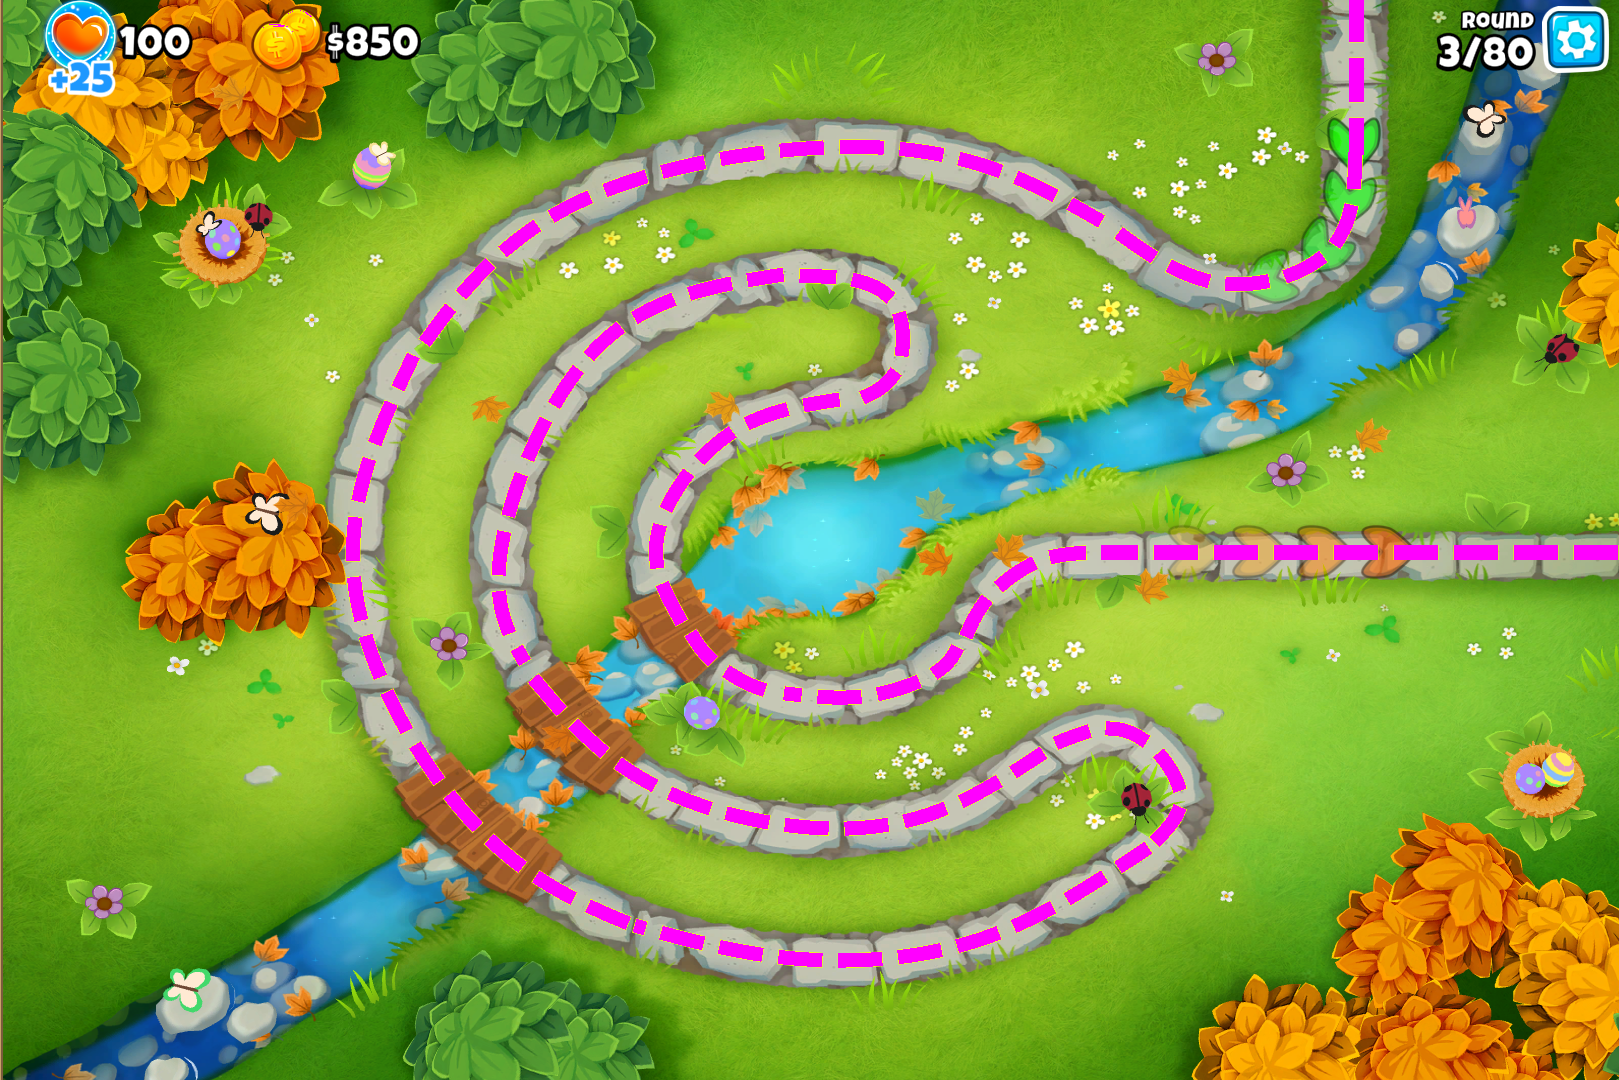
\includegraphics[width=0.95\textwidth]{img/Bloons-TD6-Park-Path-Highlighted.png}
    \end{minipage}%
    \begin{minipage}{.5\textwidth}
        \centering
        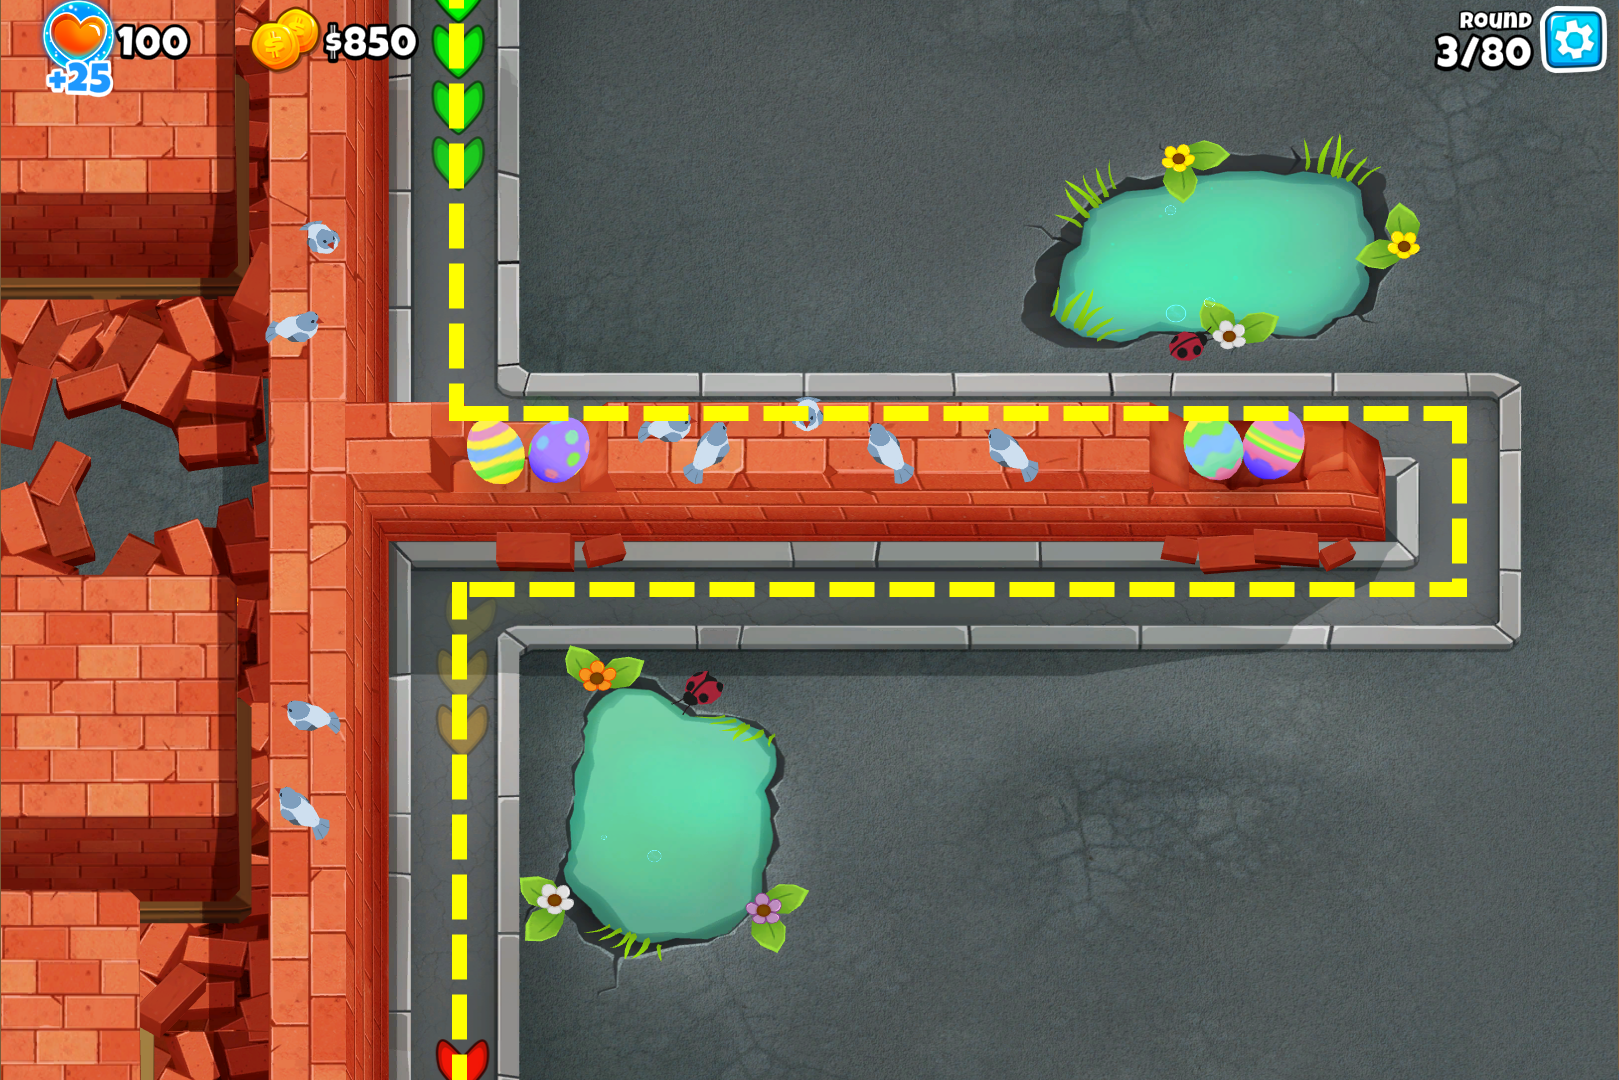
\includegraphics[width=0.95\textwidth]{img/Bloons-TD6-Another-Brick-Highlighted.png}
    \end{minipage}
    \caption{The levels \emph{Park Path} and \emph{Another Brick} from \emph{Bloons TD 6} with the attacker paths highlighted.}
    \label{fig:btd6-maps}
\end{center}

There are other options used in other games.
In \emph{Desktop Tower Defense}~\cite{DTDWiki}, for example, the attackers try to cross a rectangular playing field.
It starts out empty, but as the player fills it with towers, the attackers have to adjust their path, because they cannot go through the towers.
In figure~\ref{fig:dtd-pathfinding}, we can see the attackers funnel into a narrow passage between the defensive towers.
Since the player decides the path of the attackers, they have to learn what kind of path works well, but then they can build it all the time.
This is not ideal for us, because we want the player to adapt to the environment, not the other way around.

\begin{center}
    \captionsetup{type=figure}
    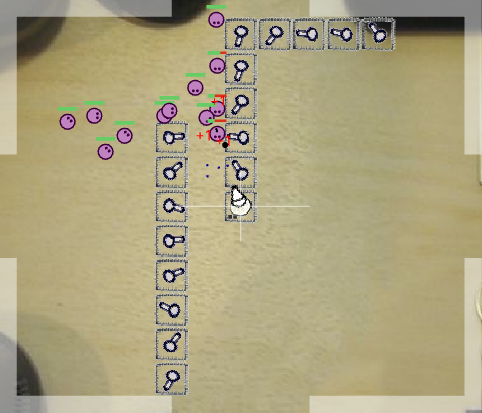
\includegraphics[width=0.6\textwidth]{img/Desktop-Tower-Defense-Playfield.png}
    \caption{Attackers being funneled between towers in \emph{Desktop Tower Defense}.}
    \label{fig:dtd-pathfinding}
\end{center}

In \emph{Plants vs.\ Zombies}, the zombies come from the right side of the screen and try to reach the left side, as we already mentioned.
The plants are planted directly in the way of the zombies and the zombies have to eat their way through them to reach their goal.
This is unique, and it greatly changes the gameplay.
However, this is again not great for our game, because we would lose a lot of potential for the levels in our game to be distinct from each other.

In \emph{Bloons TD 6}, the player receives very little information about what the upcoming waves look like.
Here, the player selects the level they want to play on, but the same sequence of waves comes every time, so the player is expected to learn at least those waves that give them problems.
In our game, however, the waves will be procedurally generated.
We want the player to plan around the upcoming waves, so we need to communicate what the upcoming waves are going to be.
This means that the waves should be simple enough to communicate effectively.
\emph{Desktop Tower Defense} features a wave preview, shown in figure~\ref{fig:dtd-waves}, that only describes the type of attacker that will come.
We want interesting behavior to emerge from the interaction of different attacker types, so we won't limit our waves to one attacker type, but instead three.
We feel that any more would make the waves messy and unnecessarily hard to communicate.

\begin{center}
    \captionsetup{type=figure}
    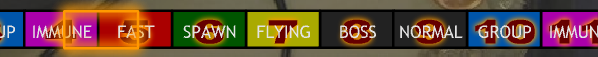
\includegraphics[width=0.8\textwidth]{img/Desktop-Tower-Defense-Waves.png}
    \caption{Wave preview from \emph{Desktop Tower Defense}.}
    \label{fig:dtd-waves}
\end{center}

In fact, each wave will be composed of one to three \emph{batches}.
Each batch will be composed of a number of attackers of only one type, spaced evenly.
Some waves will be just one batch, but this batch will send a different attacker type on each path on levels with multiple paths.
This should provide enough variety without being too hard to communicate to the player and too hard for a skilled player to predict the wave difficulty.

The waves in a single battle will get progressively harder, forcing the player will to improve their defense.
However, the wave difficulty should increase faster than the player's defense is expected to improve.
This increase will need to be carefully balanced to allow for some strategies where the player invests more into \emph{fuel} production to end a battle quickly, but also strategies where the player invests heavily into defense to keep up with the later waves.

\subsection{World}\label{sec:design-world}

In some tower defense games, for example in \emph{Desktop Tower Defense}, the towers can only be placed in positions on a grid.
In other games, for example \emph{Bloons TD 6}, the towers can be positioned freely, as long as they don't collide with each other, the attacker paths, or other obstacles.
While the second option might allow for more interesting tower placement, we will go with grid placement, and the grid will be pretty coarse~--- only $15 \times 15$ tiles.
In fact, the attacker paths will also be restricted to the grid.
They will be formed by segments, each going from the center of one tile to the center of a neighboring tile.
This is because we want the experience a player gains in one level to be transferrable to another level.
For example, they might learn that \enquote{tower A} placed right next to a straight path can handle a wave of five \enquote{attackers B} on its own.
They will then know this is true in any level whenever there is a sufficiently long straight path.
Reducing the number of path shape and tower position combinations will make the player come across a combination they already know more often, letting them predict better if their defense can handle a wave or not.
This is a really important skill to learn, because the player will have to decide before every wave, if they need to invest into defense or if they can invest into their economy.

In some tower defense games, for example in \emph{Kingdom Rush}, there are only few places where the player can place a tower in each level.
We feel this is too restrictive for our game, and it would take too much freedom away from the player.
This option also really works only in hand-crafted levels, because it is important to select the places for the towers in a way that makes for fun and interesting levels.

However, each level being just a big square of tiles with rectilinear paths on top wouldn't be very interesting.
That's why some tiles will contain obstacles that block the player from building on these tiles.
Some obstacles will be \emph{small} and some will be \emph{large}~--- they will also block the line-of-sight of towers that require a straight line between them and the attacker they want to shoot.

Another great way to make the levels more interesting, that is also intuitive for the player, is having tiles at different heights.
The heights will be in multiples of $0.5$ units, where one unit is the edge length of a tile.
Towers that require line of sight won't be able to shoot over higher terrain or down from steep cliffs.
We can also make some tower unable to shoot uphill or downhill for more variety.
Some tiles will also be slanted, gradually going from one height to another.
These tiles will allow the attacker paths to change their height, because it would be weird if the attackers had to jump up a cliff.
Some buildings will be possible to build on slanted tiles and some won't, making slants also a kind of obstacle.

As we already mentioned, each level will randomly select one of multiple \emph{terrain types}.
A terrain type will dictate how a terrain should look~--- the colors used, which terrain feature will appear and how often, and which obstacles will appear.
Each terrain type will have its distinct look, keeping the levels from being all the same.

To summarize:
\begin{itemize}
    \item The world each level takes place on will be a grid of $15 \times 15$ square tiles.
    \item There will be \emph{small} or \emph{large} obstacles on some tiles, large obstacles blocking certain towers' line of sight.
    \item The tiles will be at different heights in multiples of $0.5$ units, and some tiles will be slanted, going between two heights.
    \item Attacker paths will consist of segments going from the center of one tile to the center of a neighboring tile.
    \item The player can build one building per tile, and only if the tile doesn't contain an obstacle or the attacker path.
    \item Each world will be generated according to a randomly selected terrain type, which determines what the world will be like.
\end{itemize}

\subsection{Attacker Paths}

In subsection~\ref{sec:design-attacker-waves} we decided that the attackers will travel on predefined paths generated with the world.
If we designed each level of our game by hand, we could create paths that just feel like they would be fun to play around.
Since the paths will also be procedurally generated, we need to describe what qualities should the paths have, so the generation can later be implemented to produce such paths.

In the previous subsection we decided that the world will consist of a grid of tiles and the paths will be constrained to straight segments between the centers of the tiles.
We can think of the paths segments as one-way passages between neighboring tiles.
This means that a path cannot go twice through the same tile or cross itself, because a tile has the same path segments coming from it, no matter if it was visited for the first or second time.

There can be multiple paths in a level, each with a different shape and in some waves a different set of attackers.
This will add more variety and depth to tower placement.
Any path will also be able to split into more paths, or join together with another path, creating new path geometry or sections with different attacker density.
When a line of attackers comes to a split into multiple paths, they will alternate in which path they continue to, splitting between the paths evenly.

The player will start each level with one building already built~--- the \emph{Hub}.
It is the goal the attackers are trying to reach to destroy it.
Hence, all attacker paths will converge to the tile the \emph{Hub} is on.
The attackers will come from outside the world the battle takes place on.
The worlds are bigger, but the playable area represents just a small safe neighborhood around the \emph{Hub}.
It would be weird if the attackers just appeared on the edge tiles, so their paths will start on tiles just outside the playable world.

In figure~\ref{fig:valid-path-example} we can see an example of a valid path network drawn in blue on a world of square tiles.
The black point represents the \emph{Hub}.

\begin{center}
    \captionsetup{type=figure}
    \begin{tikzpicture}
        \draw[step=1.0,black,thin] (0,0) grid (7,7);
        \begin{scope}[blue,very thick,decoration={
                        markings,
                        mark=between positions 0.25cm and -0.15cm step 0.5cm with {\arrow{>}};
                    }]
            \draw[postaction={decorate},shift={(0.5,0.5)}] (-1,1)--(1,1)--(1,5)--(3,5)--(3,4)--(5,4);
            \draw[postaction={decorate},shift={(0.5,0.5)}] (1,2)--(3,2)--(3,1)--(5,1)--(5,4);
            \draw[postaction={decorate},shift={(0.5,0.5)}] (3,-1)--(3,1);
        \end{scope}
        \filldraw[black] (5.5,4.5) circle (5pt);
    \end{tikzpicture}
    \caption{An example of a valid path network in a $7 \times 7$ game world.}
    \label{fig:valid-path-example}
\end{center}

The attackers from single wave batch will start out evenly spaced.
If the path they are on splits into two, they will still be evenly spaced, but now the spacing is twice as large.
This is illustrated in figure~\ref{fig:attackers-path-split}, where the attackers are represented by black dots on the path.
We can also see, that after the paths join back into one, the attacker spacing is no longer even.
We don't want this to happen for aesthetic reasons, but also because overlapping attackers could be hard to identify or distinguish by the player.
This only happens when the branches of a path are of unequal length and the difference is not a multiple of the spacing between the attackers.
We don't want to put more constraints on attacker spacing, so instead, we will constrain path branches to be of equal length.
More precisely, each tile on a path has to be the same distance from the \emph{Hub}, no matter which path an attacker would take.

\begin{center}
    \captionsetup{type=figure}
    \begin{tikzpicture}
        %\draw[step=1.0,black,thin] (-0.4,0.4) grid (8.4,3.4);
        \begin{scope}[blue,very thick,decoration={
                        markings,
                        mark=between positions 0.25cm and -0.01cm step 0.5cm with {\arrow{>}};
                    }]
            \draw[postaction={decorate},shift={(0.5,0.5)}] (-1,1)--(2,1)--(2,2)--(4,2)--(4,1)--(8,1);
            \draw[postaction={decorate},shift={(0.5,0.5)}] (2,1)--(4,1);
        \end{scope}
        \filldraw (-0.3,1.5) circle (3pt);
        \filldraw (0.9,1.5) circle (3pt);
        \filldraw (2.1,1.5) circle (3pt);
        \filldraw (3.3,1.5) circle (3pt);
        \filldraw (4.5,1.5) circle (3pt);
        \filldraw (5.7,1.5) circle (3pt);
        \filldraw (6.9,1.5) circle (3pt);
        \filldraw (8.1,1.5) circle (3pt);
        \filldraw (0.3,1.5) circle (3pt);
        \filldraw (1.5,1.5) circle (3pt);
        \filldraw (2.5,1.7) circle (3pt);
        \filldraw (2.9,2.5) circle (3pt);
        \filldraw (4.1,2.5) circle (3pt);
        \filldraw (4.5,1.7) circle (3pt);
        \filldraw (5.5,1.5) circle (3pt);
        \filldraw (6.7,1.5) circle (3pt);
        \filldraw (7.9,1.5) circle (3pt);
    \end{tikzpicture}
    \caption{Attackers on a path that splits and joins.}
    \label{fig:attackers-path-split}
\end{center}

Most towers will have limited range, and they will be most effective near the attacker paths.
We want the paths to be spread out throughout the game world in order to not have tiles that are just way too far from any paths to be useful.
This is illustrated in figure~\ref{fig:path-spacing}, where we can see a path network with bad features on the left, and on the right, one with the same path lengths and starting positions, but nicer and more spread out.
We have marked tiles whose center is 2 or more tiles from the nearest path with a small cross.
In the right figure, we can also see a red point on one tile, marking a great spot for a tower.
This spot allows even a tower with shorter range, illustrated by the red ring around it, to target attackers on a large portion of the path.
On the left we have circled another U-turn in the path that is, however, undesirable.
This is because it is usually a missed opportunity for a great spot for towers.
We don't want many sharp turns like these, but they can occur from time to time for variety.
Similarly, paths going right text to each other (marked in red) are bad.
The player cannot place towers on paths, so these paths greatly limit the player's access to each other, making for an unpleasant experience.

\begin{center}
    \captionsetup{type=figure}
    \begin{tikzpicture}
        \draw[step=1.0,black,thin] (0,0) grid (6,6);
        \draw[step=1.0,black,thin] (7,0) grid (13,6);
        \begin{scope}[blue,very thick,decoration={
                        markings,
                        mark=between positions 0.25cm and -0.15cm step 0.5cm with {\arrow{>}};
                    }]
            \draw[postaction={decorate},shift={(0.5,0.5)}] (2,6)--(2,5)--(1,5)--(1,4)--(4,4);
            \draw[postaction={decorate},shift={(0.5,0.5)}] (5,6)--(5,4);
            \draw[red,postaction={decorate},shift={(0.5,0.5)}] (4,4)--(4,1);
            \draw[red,postaction={decorate},shift={(0.5,0.5)}] (5,4)--(5,1);
            \draw[postaction={decorate},shift={(0.5,0.5)}] (5,1)--(3,1);
            \draw[postaction={decorate},shift={(0.5,0.5)}] (9,6)--(9,4)--(7,4)--(7,2)--(9,2)--(9,1)--(10,1);
            \draw[postaction={decorate},shift={(0.5,0.5)}] (12,6)--(12,3)--(11,3)--(11,1)--(10,1);
        \end{scope}
        \filldraw[black] (3.5,1.5) circle (5pt);
        \filldraw[black] (10.5,1.5) circle (5pt);
        \draw (0.5, 0.5) node[cross=2.5pt] {};
        \draw (0.5, 1.5) node[cross=2.5pt] {};
        \draw (0.5, 2.5) node[cross=2.5pt] {};
        \draw (1.5, 0.5) node[cross=2.5pt] {};
        \draw (1.5, 1.5) node[cross=2.5pt] {};
        \draw (1.5, 2.5) node[cross=2.5pt] {};
        \draw[red] (2,5) circle (0.8cm);
        \filldraw[red] (8.5,3.5) circle (4pt);
        \draw[red] (8.5,3.5) circle (1.6cm);
    \end{tikzpicture}
    \caption{A path network with undesirable properties and a path network with great properties.}
    \label{fig:path-spacing}
\end{center}

In relation to this, we will also ban all path branches that join back to the original path after less than 4 path segments.
They necessarily produce paths right next to each other, as illustrated on figure~\ref{fig:too-short-path-splits}, which don't express the properties that make path splits interesting, and just take up more space unnecessarily.

\begin{center}
    \captionsetup{type=figure}
    \begin{tikzpicture}
        \begin{scope}[blue,very thick,decoration={
                        markings,
                        mark=between positions 0.25cm and -0.01cm step 0.5cm with {\arrow{>}};
                    }]
            \draw[postaction={decorate},shift={(0.5,0.5)}] (0,2)--(2,2)--(2,1)--(5,1)--(5,2)--(6,2)--(6,1)--(7,1)--(7,2)--(8,2);
            \draw[postaction={decorate},shift={(0.5,0.5)}] (1,2)--(1,1)--(2,1);
            \draw[postaction={decorate},shift={(0.5,0.5)}] (3,1)--(3,2)--(5,2);
            \draw[postaction={decorate},shift={(0.5,0.5)}] (6,2)--(6,3)--(7,3)--(7,2);
        \end{scope}
        \draw[blue] (2,2) node{\textbf{2}};
        \draw[blue] (4.5,2) node{\textbf{3}};
        \draw[blue] (7,2.5) node{\textbf{3}};
    \end{tikzpicture}
    \caption{All the path splits which join back after less than 4 path segments.}
    \label{fig:too-short-path-splits}
\end{center}

To summarize, these are the rules the paths should follow:
\begin{itemize}
    \item Paths are formed by one-way segments, each from one tile to its neighbor.
    \item Paths start just outside the playable portion of the world, and there can be one or more path starts in each level.
    \item Paths can split or join.
    \item All paths must end on the tile with the \emph{Hub}, no other dead ends can exist.
    \item Each tile on a path has to be the same distance from the \emph{Hub}, no matter which path an attacker would take.
    \item Paths should be spread throughout the playable world, not bunched up.
    \item Paths right next to each other and sharp U-turns (viz figure~\ref{fig:path-spacing}) should be rare.
    \item No path branches can join back to the original path after less than 4 path segments.
\end{itemize}

\section{Attacker Types}

We have mentioned that there will be many attacker types in out game.
Each will be designed on its own, but they will be randomly combined to make attacker waves.
An attacker type defines the following properties of an attacker:
\begin{itemize}
    \item \textbf{Appearance}. Every attacker will be represented in a battle by its 3D model, corresponding animations and other visual effects. Every attacker type will also have an associated icon to display in the user interface.
    \item \textbf{Hit Points} or \textbf{HP} determine how much damage can an attacker take from the towers before it dies.
    \item \textbf{Movement speed} in tiles per second.
    \item \textbf{Size}~--- either \emph{small}, \emph{large} or \emph{boss}~--- determines how much \emph{hull} (see section~\ref{sec:design-hull}) the player loses when this attacker reaches the \emph{Hub}. Also defines the height off the ground of the spot defensive towers target. More details below.
    \item \textbf{Abilities}. These can be \emph{passive} (for example \enquote{Immune to fire.}), \emph{repeating} (\enquote{Heals 5\,HP every two seconds.}), or \emph{reactive} (\enquote{Spawns \emph{attacker A} when killed.}).
\end{itemize}

The height of a target a tower shoots at is important~--- lower targets can easily hide behind a terrain feature or an obstacle.
We want some attackers to look bigger than others, and it would be weird if the towers shot at a lower portion of their model.
Larger attackers will have their targeting point higher.
To make things simple for the player, there are only two heights of the targeting point~--- \emph{small} at $0.15$ units above the ground and \emph{large} at $0.3$.

Whenever an attacker reaches the \emph{Hub}, the player will lose some \emph{hull}.
The \emph{small} attackers will come in greater numbers than \emph{large} attackers.
To make the stakes more equal, \emph{small} attackers cost the player only 1 hull, whereas the \emph{large} attackers cost 3 hull.

The player will encounter only few \emph{boss} attackers in every run.
They will be the main attackers in special boss levels, which are spread throughout the run and cannot be avoided by the player.
When a boss reaches the \emph{Hub}, the player immediately loses the game.
Each boss will bend the rules of the game a bit as one of their abilities, but most of them will have the same target height as \emph{large} attackers.

\subsection{Buildings}

As stated, the player will be able to build buildings, but only between waves of attackers.
They will be able to build one building per tile, if the tile has no obstacles and an attacker path is not going through it.
Each building costs some amount of \emph{materials} to build.
The player will be able to delete a building at any time, mainly to make way for other buildings.

There are three building types defined by their primary function: \emph{towers}, \emph{economic} and \emph{special}.
Towers kill or otherwise impede attackers, and economic buildings produce resources.
Special buildings are the buildings that don't fit in either category.
They usually have a unique ability, for example for increasing the effectiveness of other buildings.
Economic buildings often produce resources at the end of every wave, just in time for the player to use them to build more buildings.
However, some economic buildings produce resources at other times, often as a reaction to some other event, for example an attacker dying.

One notable special building is the \emph{Hub}, since the player starts each level with one for free, and they cannot build more.
The goal of the attackers is to reach the \emph{Hub}, and when they do, the player loses some \emph{hull} (viz section~\ref{sec:design-hull}).
Additionally, the \emph{Hub} produces some amount of \emph{fuel}, \emph{materials} and \emph{energy} at the end of each wave.
These resources are further described in their respective sections.

\subsection{Towers}

Towers are the buildings which kill or otherwise impede attackers.
There are many properties that distinguish towers from each other.
There is a lot of freedom to allow for many unique designs.
Combining towers with different properties is supposed to be a fun and interesting part of the game.

Towers usually shoot once per their \emph{shot interval}, but some towers can shoot multiple projectiles at once, others deal a certain amount of damage per second continuously.
They can usually only target attackers in a circular range around them.
However, some towers have an unlimited range, or their range is not circular.
Most towers instantly aim at their target, some take time to rotate around and others cannot rotate at all.
Some towers cannot aim upwards or downwards.
Most towers require line of sight to their target, but some don't.
Most towers fire projectiles in a straight line, but some don't fire projectiles, others fire projectiles that travel over obstacles along a ballistic arc.
Some towers can even miss their target.
With tower designs, the sky is the limit.

Whenever a tower has more attackers in its range, it will decide which one to target based on the tower's targeting priority.
The player will be able to select one of these priorities on most towers:
\begin{itemize}
    \item First~--- the attacker that's closest to the \emph{Hub}.
    \item Last~--- the attacker that's farthest from the \emph{Hub}.
    \item Closest~--- the attacker that's closest to this tower.
    \item Farthest~--- the attacker that's farthest from this tower.
    \item Strongest~--- the attacker with the greatest HP.
    \item Weakest~--- the attacker with the least HP.
\end{itemize}
This will let the player have more control over their towers, allowing them to best use their unique properties.

The damage the towers deal come in many types.
For example \emph{physical}, \emph{fire}, \emph{explosive}, \emph{electric}.
Some towers will deal damage of multiple types at once.
This distinction lets us make some towers explicitly weak against some attackers~--- those that are resistant to the given damage type.
Or it lets us restrict some synergies, for example by making a building that makes attackers take more damage from \emph{electricity} only.

It is worth mentioning, that in most tower defense games, the player can upgrade any tower during a battle by investing more resources into it.
The upgrades often increase a tower's damage or fire rate, however some substantially change the tower's behavior.
Some games take this to the extreme, for example in \emph{Bloons TD 6}, each tower has 15 different upgrades available, and each tower can be upgraded to two different upgrades at once.
However, in our game, the player won't be able to upgrade their towers during a battle.
Instead, they will have to have some towers that are useful at the start of a level, and others that are more powerful, but more expensive, to be used later.

\subsection{Abilities}\label{sec:design-abilities}

- used mid-wave

- usually instant effects

- free placement, global placement, tile placement, use on a building


\subsection{Materials and energy}\label{sec:design-materials-and-energy}

- what, why, consequences and constraints

- separation of materials and energy

\subsection{Fuel}\label{sec:design-fuel}

- win the game

\section{Battle Graphical User Interface}

\xxx{specify controls, use images}

\subsection{Waves Left and Fuel}

- and time controls

\subsection{Hull}\label{sec:design-hull}

\subsection{Wave Preview}

\subsection{Materials and Energy}

\subsection{Blueprints}

- separate blueprint menu and blueprint design

- what they represent

- limited number

- cost and cooldowns

- rarities

- how are they obtained

- make them unique

- break the rules (build on paths, ability to make buildings ...)

- lenticular design

- blueprint upgrades

\subsection{Info Panel and Selection}

- what it looks like and what's on it

- select blueprints

- select buildings

- select attackers

- dynamic values

\subsection{Highlights and Range Visualization}

\section{Camera controls}

- zoom to look closely, rotate so the terrain doesn't hide stuff

\section{Future Features}

- setting

- run structure

- map

- events and shops

- saving the game

- unlocks

- difficulty levels
